\section{Présentation de l'étude\label{section:pres}}

Pour ce projet, nous nous intéressons à la perte de pression ainsi qu'au taux de vide moyen pour un écoulement bouillant dans une conduite chauffée. Une représentation d'un banc d'essai typique pour ce type de mesures est disponible à la fig. \ref{fig:instal}

\begin{figure}[htbp]
    \centering
    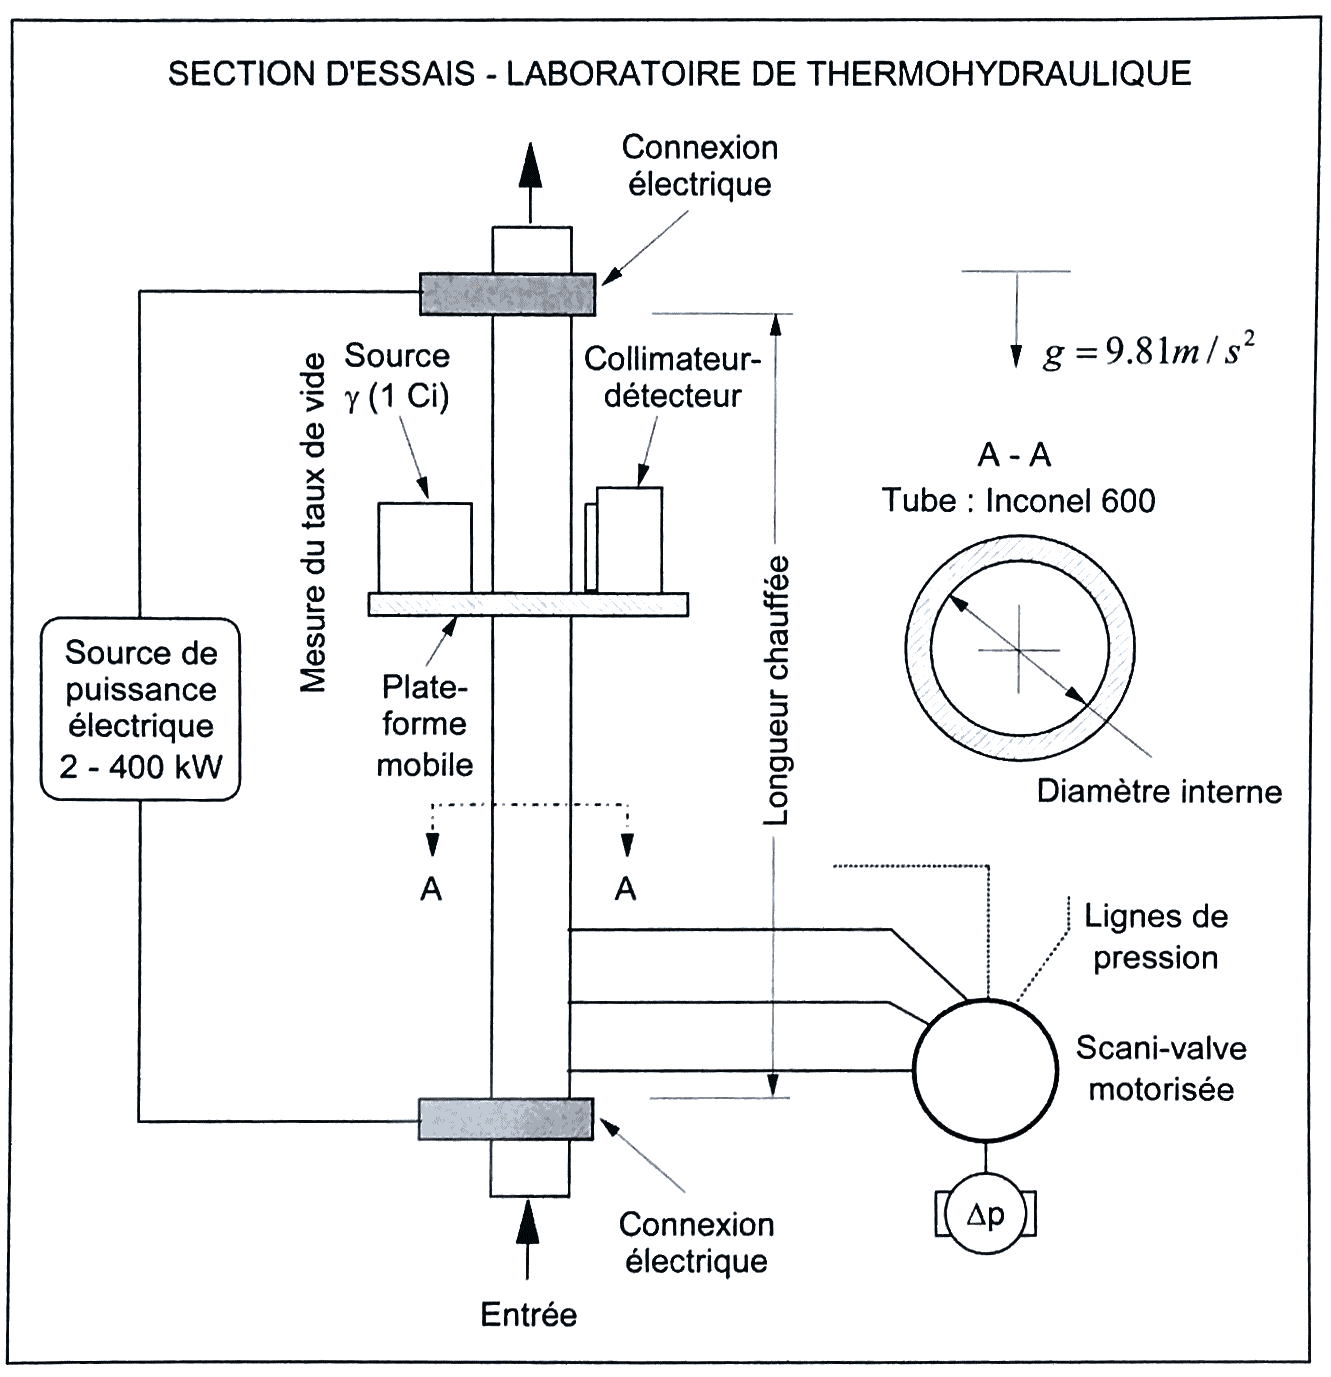
\includegraphics[width=0.8\textwidth]{images/schema_instal.png}
    \caption{Installation pour mesure de perte de pression et du taux de vide - D'après l'énoncé}
    \label{fig:instal}
\end{figure}

Le but de ce projet est de réaliser un modèle numérique et de déterminer les différents paramètres le long de la conduite. L'analyse des résultats se fait en comparant à des tables de données expérimentales. On travaille dans le cas d'un écoulement vertical ascendant.\\ \par
Pour réaliser cela, plusieurs hypothèses ont été réalisées :
\begin{itemize}
    \item \textbf{H1} : L'écoulement est incompressible.
    \item \textbf{H2} : La perte de pression par accélération dans la région non bouillante est négligeable.
    \item \textbf{H3} : La perte de pression totale est négligeable par rapport à la pression de l'écoulement.
\end{itemize}
\vspace{12pt}
\par
La détermination des propriétés thermodynamiques a été faite avec \texttt{pyXSteam}, qui est une librairie Python sur la base de \texttt{X-Steam} disponible sur Excel et Matlab.\\
Le titre et le taux de vide moyen sont déterminés à l'aide des corrélations de \textsc{Chexal-Lellouche}. Le multiplicateur diphasique ainsi que les facteurs de frottements qui servent au calcul de la perte de pression proviennent eux de la corrélation de \textsc{Friedel}.\\ \par
\textcolor{red}{A voir si on met l'explication de travailler avec TensorFlow, je pense que cela peut-etre interessant. On aura le temps de reprendre cela.}
